\documentclass[]{interact}

\usepackage{caption}
\captionsetup{font=normalsize}
\usepackage{subcaption}

\begin{document}

% \begin{figure}
%     \centering
%     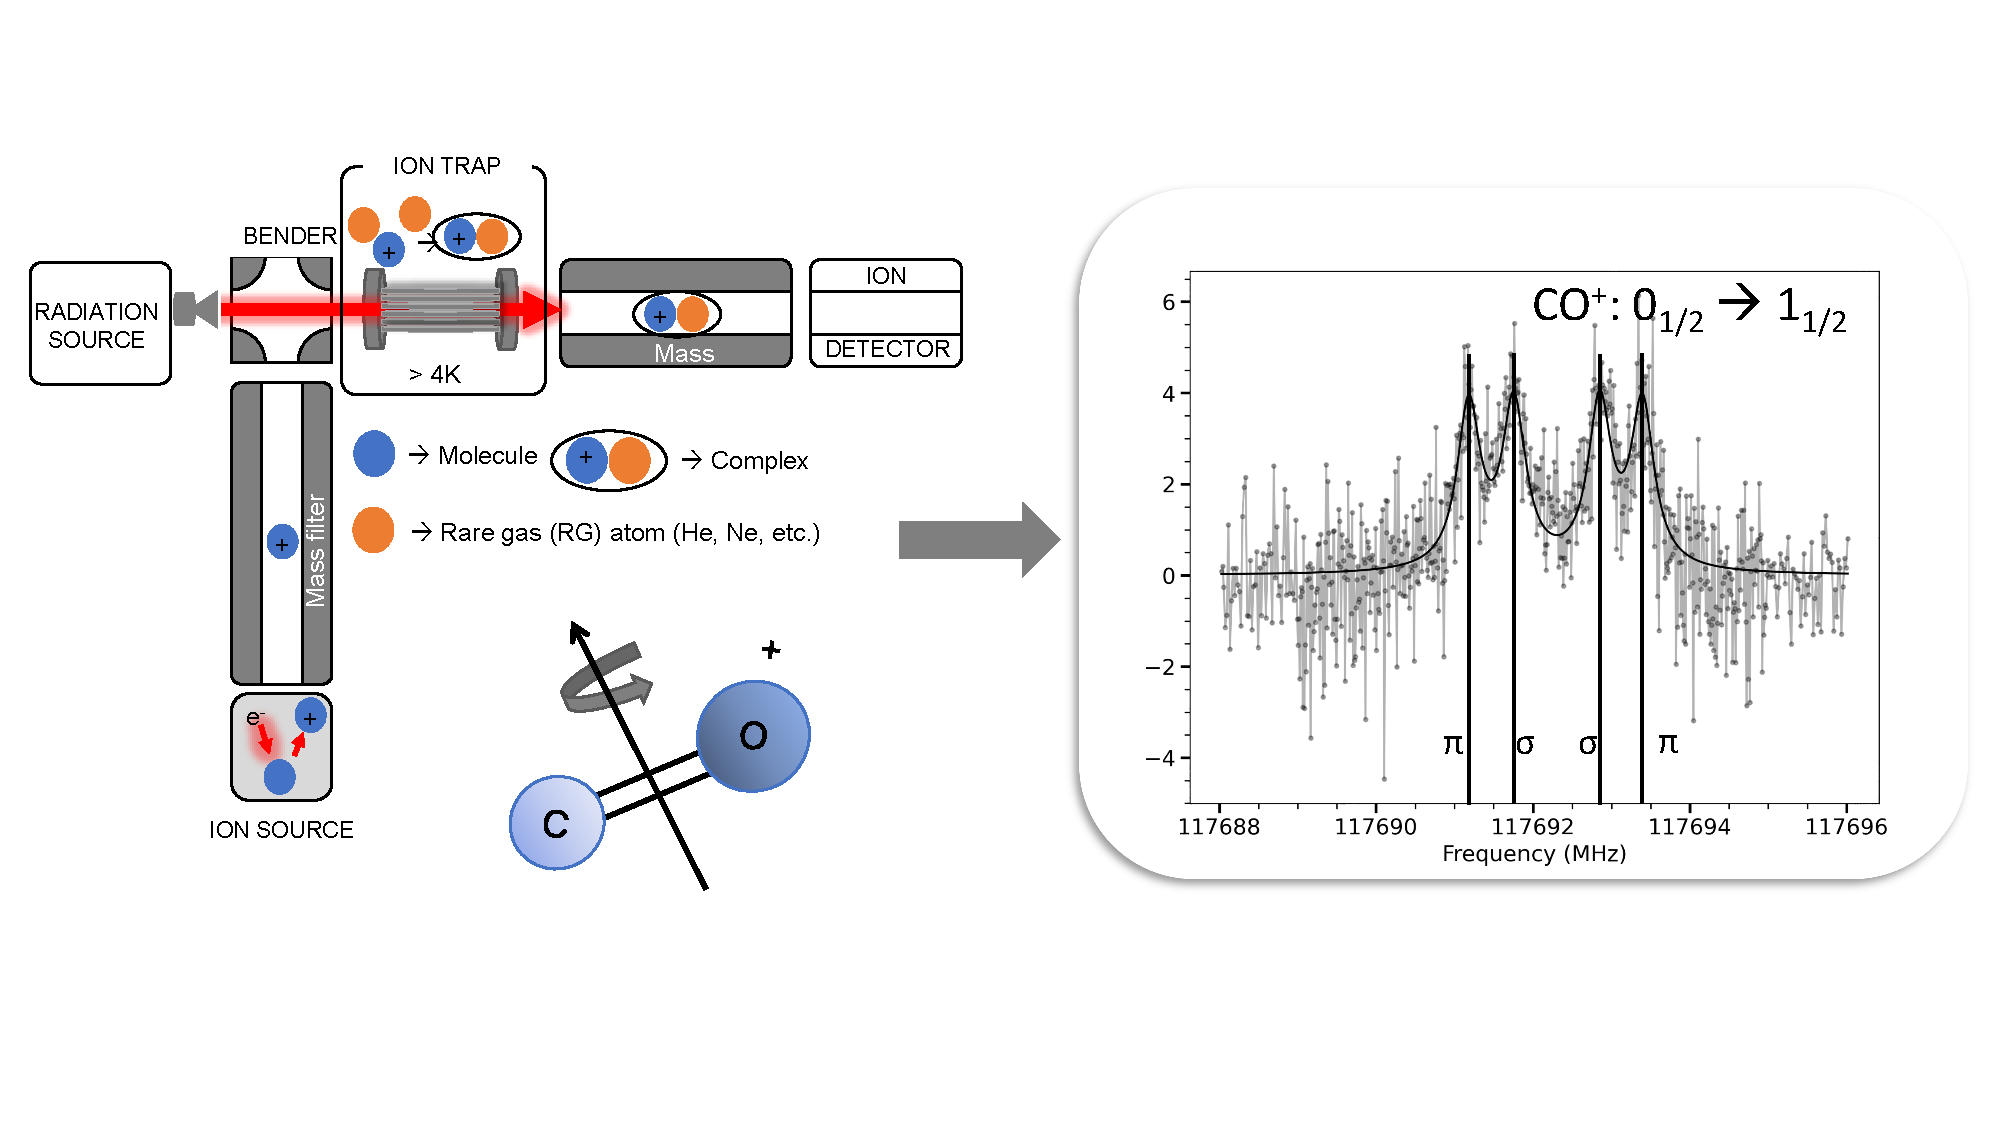
\includegraphics[scale=0.5]{GA/CO+_graphicalAbstract.pdf}
%     \caption{GA}

% \end{figure}

RULES:\\ For compatibility with our peer review systems, please submit
electronic artwork files in one of our

preferred formats:
\begin{enumerate}
    \item EPS
    \item  PS
    \item JPEG
    \item TIFF
    \item Microsoft Word (DOC or DOCX only)
\end{enumerate}
Please do not supply files in PDF format because these are ‘locked’ files and incompatible with our
workflow software

Search engines cannot easily read text in image-based files such as JPEG, BMP,
PNG etc. after indexing. This makes it difficult for caption-text, graphs,
tables, and keywords included in a graphical abstract to be discovered online.
If you are submitting artwork which includes text, please use one of the
following formats:
\begin{enumerate}
    \item EPS
    \item  PS
\end{enumerate}

PostScript and Encapsulated PostScript should be high-resolution and all fonts
should be embedded. Minimum line weight is 0.3pt for black lines on a white
background. This is the recommended format for line art, combinations of
photographs, and labeling.

\begin{figure}
    \centering
    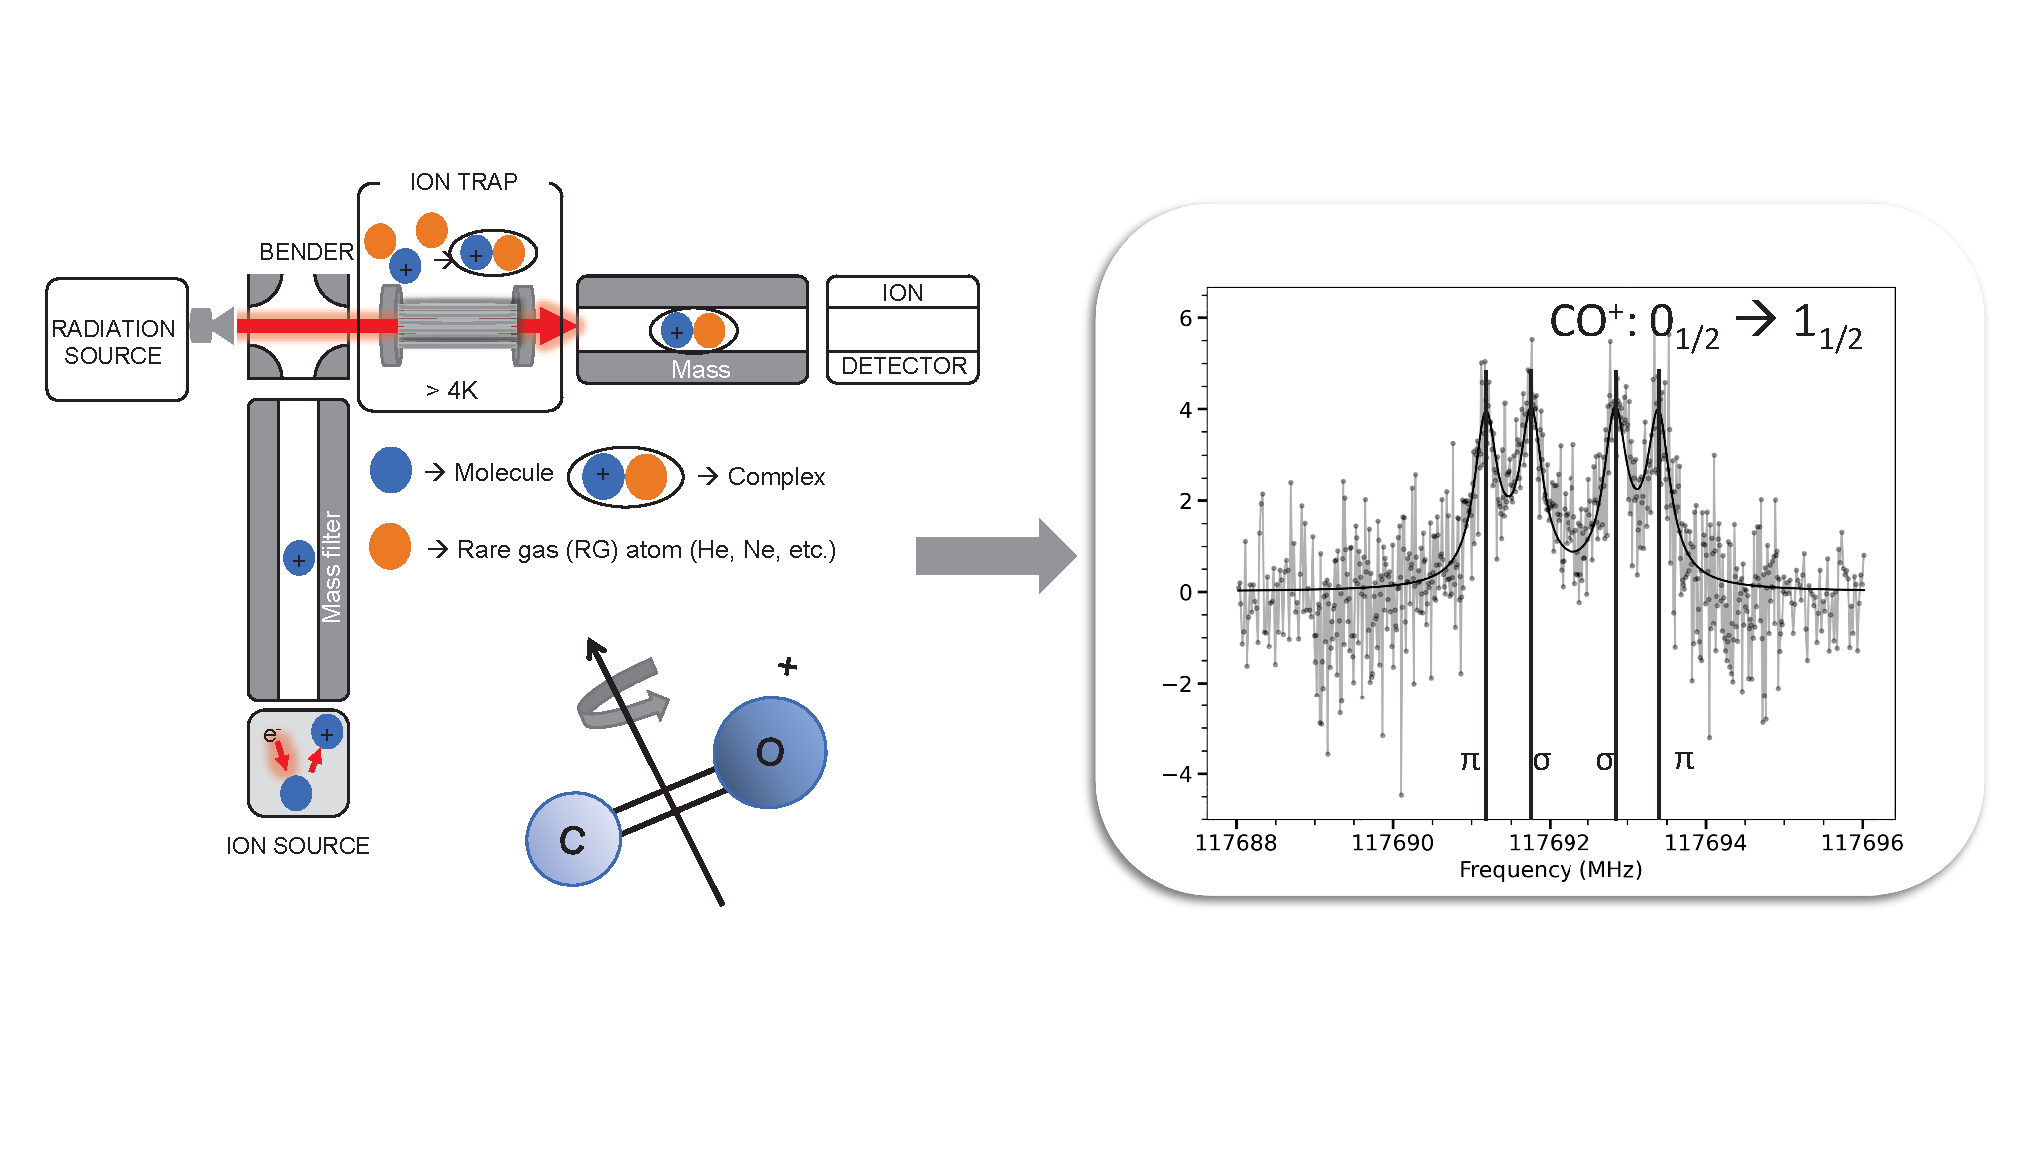
\includegraphics[scale=0.5]{GA/CO+_graphicalAbstract.eps}
    \caption{CO$^+$: Graphical abstract (EPS format)}
\end{figure}
\end{document}